\hypertarget{part-2-image-2}{%
	\section{Part 2, Image 2}\label{part-1-design-3}}

\centering


\hypertarget{description}{%
	\subsubsection{Description}\label{description}}

\begin{description}
	\item[Image:]
	\item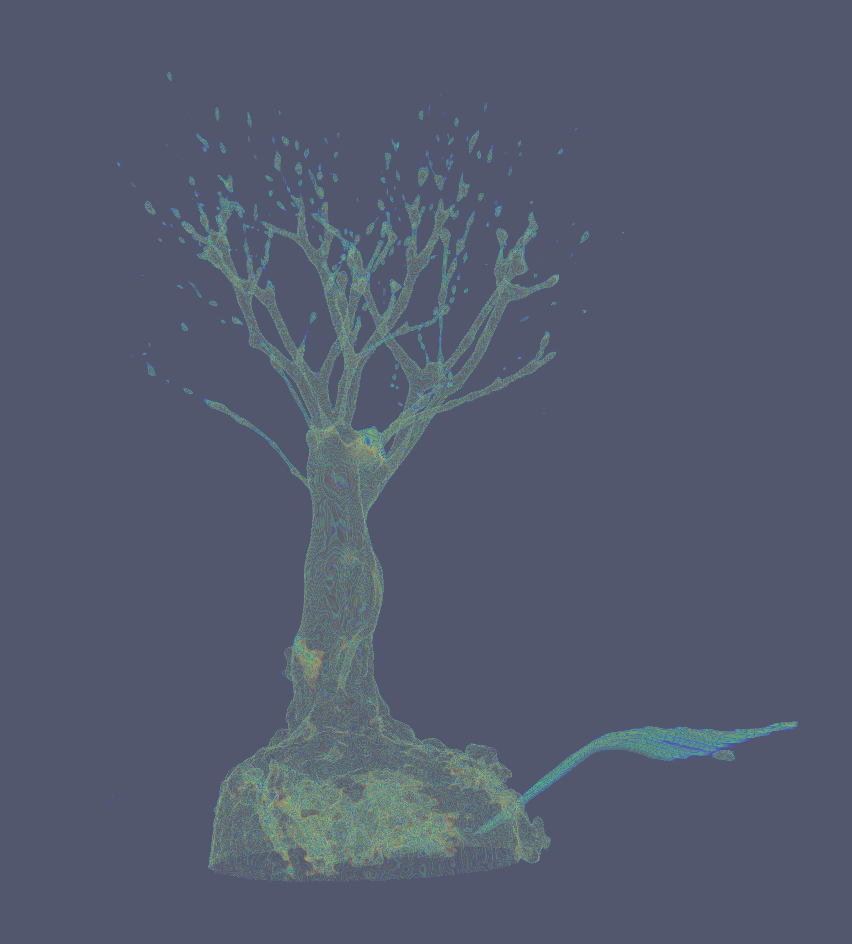
\includegraphics[width=10cm]{Tree2.png}
	\item[Tool:]
	\hfill \break
	Paraview
	\item[Visual Mappings:]
	\begin{itemize}
		\tightlist
		\item[ ]
	\end{itemize}
	\begin{itemize}
		\tightlist
		\item
		\textbf{Mapping 1}:
		\hfill \break 
		Colour mapping is set to LAB.
	\end{itemize}
	
	\begin{itemize}
		\tightlist
		\item
		\textbf{Mapping 2}:
		\hfill \break 
		Data point 128.692 has been set to brown with an opacity of 0.608, while datapoint 27 has been set to green with an opacity of 0.000.
	\end{itemize}
	\item[Data Conversion:] 
	\hfill \break 
	Data scalar type unsigned char was used. Along with data extent: 0 - 511, 0 - 511, 0 - 181. Representation is volume. Data byte order is BigEndian with a file dimensionality of 3. Ray tracing rendering has been enabled, with an OSPRay raycaster set and the blend mode is Isosurface. Value ranges in the volume rendering have been set to 127.5 and 27.
	\item[Unique Observation:]
	\hfill \break 
	The inside of the tree trunk is at value 127.5, which is depicted in the brown colour in the image. However, the other layer of the tree, with the leaves are at value 27 show green on the visualisation. When using an Isosurface blend mode, opacity does not have an effect on how to colour is represented in the visualisation.
	
	%At data point 76.894 is where the internal part of the tree trunk disappears. While at data point 54.696, this is where the leaves will start to disappear from the visualisation.
	
\end{description}